% Metaphor: control loop. The output comes back round and changes the
% next input -- reach for it when the figure's whole claim is that the
% cycle closes. If nothing returns, this is a pipeline.
%
% Idiom: cyclic edges with `bend`. The bend is what makes the return
% path read as a return path rather than as a line that happens to run
% backwards; nodes are placed relative to each other with `positioning`
% so the cycle keeps its shape when a label grows.
\usetikzlibrary{positioning}
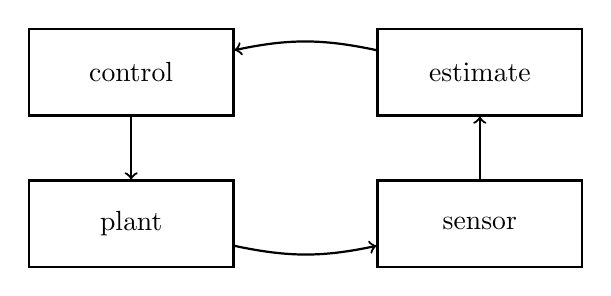
\begin{tikzpicture}[thick,
                    unit/.style={draw,align=center,
                                 minimum width=26mm,minimum height=11mm}]
  \node[unit] (plant) {plant};
  \node[unit,right=18mm of plant] (sensor) {sensor};
  \node[unit,above=8mm of sensor] (estimate) {estimate};
  \node[unit,above=8mm of plant] (control) {control};
  % `bend right` on both horizontal edges, so each bows *away* from the
  % centre. Bending them the other way is the easy slip: the two curves
  % then lean into the middle of the loop and read as one lens-shaped
  % blob rather than as a cycle going round.
  \draw[->] (plant) to[bend right=12] (sensor);
  \draw[->] (sensor) -- (estimate);
  \draw[->] (estimate) to[bend right=12] (control);
  \draw[->] (control) -- (plant);
\end{tikzpicture}
